\documentclass[12pt, a4paper]{article}
\usepackage[utf8]{inputenc}
\usepackage[T1]{fontenc}
\usepackage{geometry}
\geometry{a4paper, margin=2.5cm}
\usepackage{amsmath, amssymb}
\usepackage{graphicx}
\usepackage{booktabs}
\usepackage{hyperref}
\usepackage{setspace}
\usepackage{authblk}
\usepackage{float}
\usepackage{titlesec}
\usepackage{lmodern}

% Aesthetic touches
\titleformat{\section}{\large\bfseries}{\thesection}{1em}{}
\onehalfspacing

\title{\textbf{Networks Decide for Us: \\ Emergence of Adoption in Homophily-Imputed Social Topologies}}

\author[1]{Aníbal Olivera-Morales\thanks{Corresponding author: \texttt{an.oliveram@udd.cl}}}
\author[1]{Jorge Fábrega-Lacoa}
\author[2]{Thomas W. Valente}

\affil[1]{Centro de Investigación en Complejidad Social, Universidad del Desarrollo, Santiago, Chile}
\affil[2]{Department of Population and Public Health Sciences, Keck School of Medicine, University of Southern California, Los Angeles, USA}

\date{\today}

\begin{document}

\maketitle

\begin{center}
    \textit{Extended Abstract submitted to the Social Networks Special Issue: \\ ``Agent-Based Modelling for Social Network Research''}
\end{center}

\vspace{1cm}

\section*{Research Question}
The diffusion of innovations, social norms, and collective behaviors is frequently modeled as either a result of individual utility maximization or a contagion process. However, empirical reality suggests a hybrid mechanism where individuals weigh both their intrinsic preferences and the influence of their peers. Furthermore, the structure of these peer networks is rarely random; it is shaped by deeply ingrained homophilic forces.

This research asks: \textit{To what extent does the structure of social networks, shaped by empirical homophily, independently govern the diffusion of collective behaviors, conditional on fixed individual-level propensities?} We propose that the level of adoption in a society is an emergent property of the relational structure, not just the aggregate of individual wills. We advance the claim that ``networks decide for us'': the topological arrangement itself acts as a non-neutral scaffold that actively enables or constrains social change.

\section*{Data}
To build realistic network structures, we combine representative survey data with empirical homophily parameters. First, we use the homophily targets estimated by McPherson and Smith (2019) from the General Social Survey (GSS 2004) core discussion networks module, spanning dimensions of Blau space such as Age, Sex, Education, Race, and Religion. Second, we impute these relational structures onto $1000$ respondents from the American Trends Panel (ATP 2016). While the respondents providing the network parameters (GSS) are different from those providing the individual propensities for collective action (ATP), this imputation allows us to generate a large set of structural replicates. The resulting topologies respect the marginal demographic distributions while adhering to empirical homophily tendencies, producing realistic clustering and degree distributions that overcome the limitations of standard random network models.

\section*{Methods: Hybrid Agent-Based Modeling}
We analyze diffusion processes over these imputed topologies using a hybrid Agent-Based Model (ABM) that integrates \textit{Rational Choice} and \textit{Selective Social Influence}. The process, simulated using the \texttt{netdiffuseR} package (Vega Yon, Olivera Morales, \& Valente, 2025), initializes by distributing a behavioral innovation. In our model, agents adopt intrinsically if the innovation's utility exceeds their individual required threshold (Rational Adoption). Alternatively, agents adopt through peer contagion if exposed to a critical mass of adopters who are socially proximate (Social Adoption). Crucially, the influence of peers is weighted by social similarity (Gower's distance), constrained by a Maximum Social Proximity ($MSP$) parameter. 

Through extensive simulations ($\approx 4$ million runs), we explore the parameter space of intrinsic utility and social flexibility across both our Plausible networks and Erdős-Rényi (Random) baselines. Total Adoption represents the combined effectiveness of individual incentives and structural mobilization.

To isolate the marginal effect of network structure on emergent outcomes, we employ Big Additive Models (BAM), a scalable implementation of Generalized Additive Models (GAMs). These models allow us to estimate the isolated effects of Ratonal, Social, and Total Adoption. The BAMs include thin-plate regression splines $s(IUL, MSP)$ to capture the non-linear interacton between intrinsic utility and social flexibilty, while controlling for threshold distribution parameters and network structure.

\section*{Preliminary Findings}
By comparing the diffusion outcomes on Plausible networks against their Random baselines, we quantify the ``structural premium'' of realistic network topologies. Our Generalized Additive Models (BAM) regressions reveal several key dynamics:

\begin{enumerate}
    \item \textbf{The Structural Premium:} Randomizing the network structure significantly depresses overall adoption. The specific clustering and homophilic segregation inherent in realistic networks facilitate behavioral cascades that random networks cannot sustain. Under random conditions, the odds of total adoption are drastically reduced (BAM coefficient = -0.850, $p < 0.001$).
    \item \textbf{Non-Linear Phase Transitions and Empirical Criticality:} We identify distinct interaction regimes between intrinsic utility ($\Gamma$) and social flexibility ($h$). When the population is highly rigid (low MSP), homophilic echo chambers freeze the network, stifling diffusion regardless of utility. As flexibility increases, a sharp ``tipping point'' emerges where social reinforcement overcomes localized resistance. We validate the continuous (second-order) nature of this transition using three independent methods inspired by statistical physics: (a) \textit{Critical Slowing Down (CSD)}: the standard deviation of simulation relaxation times diverges precisely along the critical boundary, and Pearson correlations between total adoption and relaxation time shift from near-zero ($r \approx 0.24$) in the rigid sub-critical phase to strongly negative ($r \approx -0.89$) in the fluid super-critical phase; (b) \textit{Avalanche Distributions}: exactly at the susceptibility peak ($MSP_c \approx 0.58$), cascade sizes follow a violent bimodal distribution---diffusion either collapses microscopically or triggers system-wide adoption in 900+ nodes---a hallmark of scale-free criticality absent in random-network baselines; (c) \textit{Critical Exponents}: using the Fluctuation-Dissipation Theorem to compute susceptibility as $\chi = \text{Var}(\Phi)$, we recover an empirical susceptibility exponent $\gamma \approx 0.977$ ($\pm 0.01$) along the Widom Line, an extraordinary match to the Mean-Field Ising prediction ($\gamma = 1.0$), placing collective social adoption in a mathematically rigorous universality class.
    \item \textbf{The Role of Selective Influence:} The data shows that ``who we are'' is inextricably linked to ``who we know,'' but the structural pathway dictates the outcome. Our findings directly challenge models assuming uniform influence, emphasizing that homophily operates as a dynamic gate for diffusion.
\end{enumerate}

Our results demonstrate that applying ABM to empirically calibrated network topologies uncovers macro-social outcomes that statistical aggregations miss. Unlike traditional statistical frameworks such as Exponential Random Graph Models (ERGMs) or Stochastic Actor-Oriented Models (SAOMs)---which may face computational tractability issues or rely on assumptions of perfectly rational actors---our ABM approach directly captures the non-linear micro-macro feedback cycles. By operationalizing homophily not just as a structural feature but as a dynamic gate for influence, we identify causal mechanisms with greater precision, proving that network topology acts as an autonomous engine for coordination in social systems. The findings contribute to social network research by illustrating that network structure is a fundamental causal mechanism in the dynamic unfolding of collective behavior.

\newpage

\section*{Illustrative Evidence}

\begin{figure}[H]
    \centering
    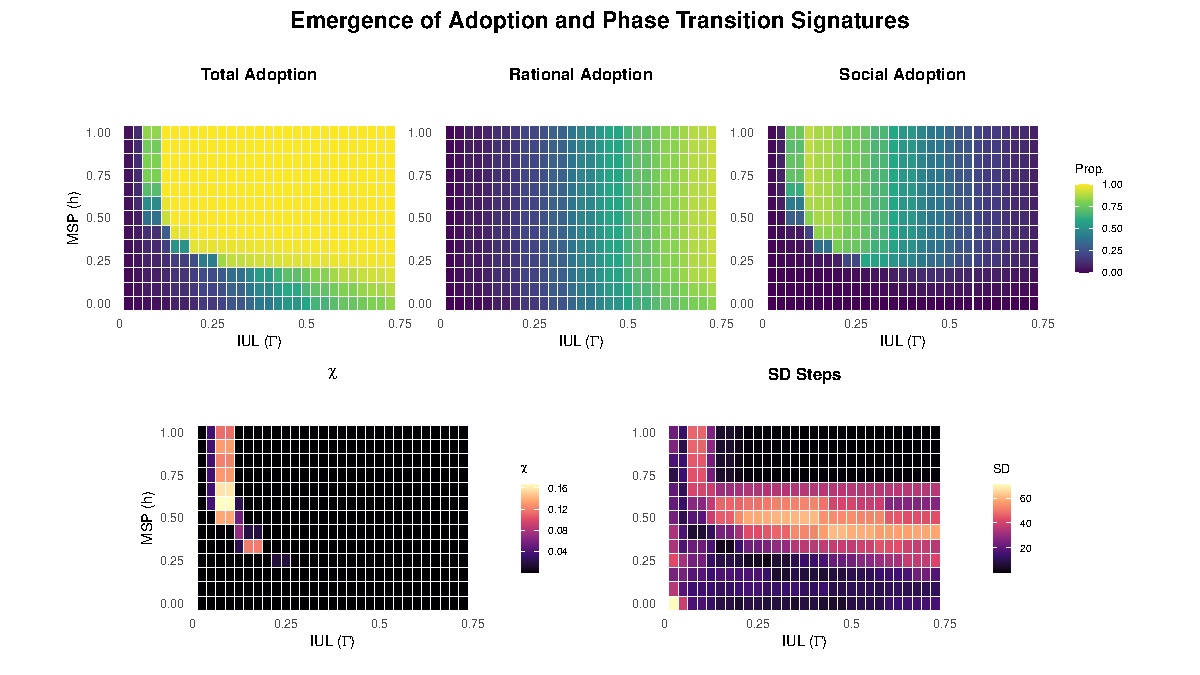
\includegraphics[width=1\textwidth]{figure1_5panels_GSS.pdf}
    \caption{\textbf{Adoption Regimes and Phase Transition Signatures.} \textit{Top row:} Average Total, Rational, and Social Adoption heatmaps. \textit{Bottom row (left):} Susceptibility $\chi = \text{Var}(\Phi)$ via the Fluctuation-Dissipation Theorem, with the phase boundary visible as a ridge of high variance. \textit{Bottom row (right):} Standard Deviation of simulation relaxation time; its divergence along the critical boundary is the signature of Critical Slowing Down. Simulations based on a GSS plausible network, $\tau_{sd}=0.12$, and random seeding.}
\end{figure}

\begin{figure}[H]
    \centering
    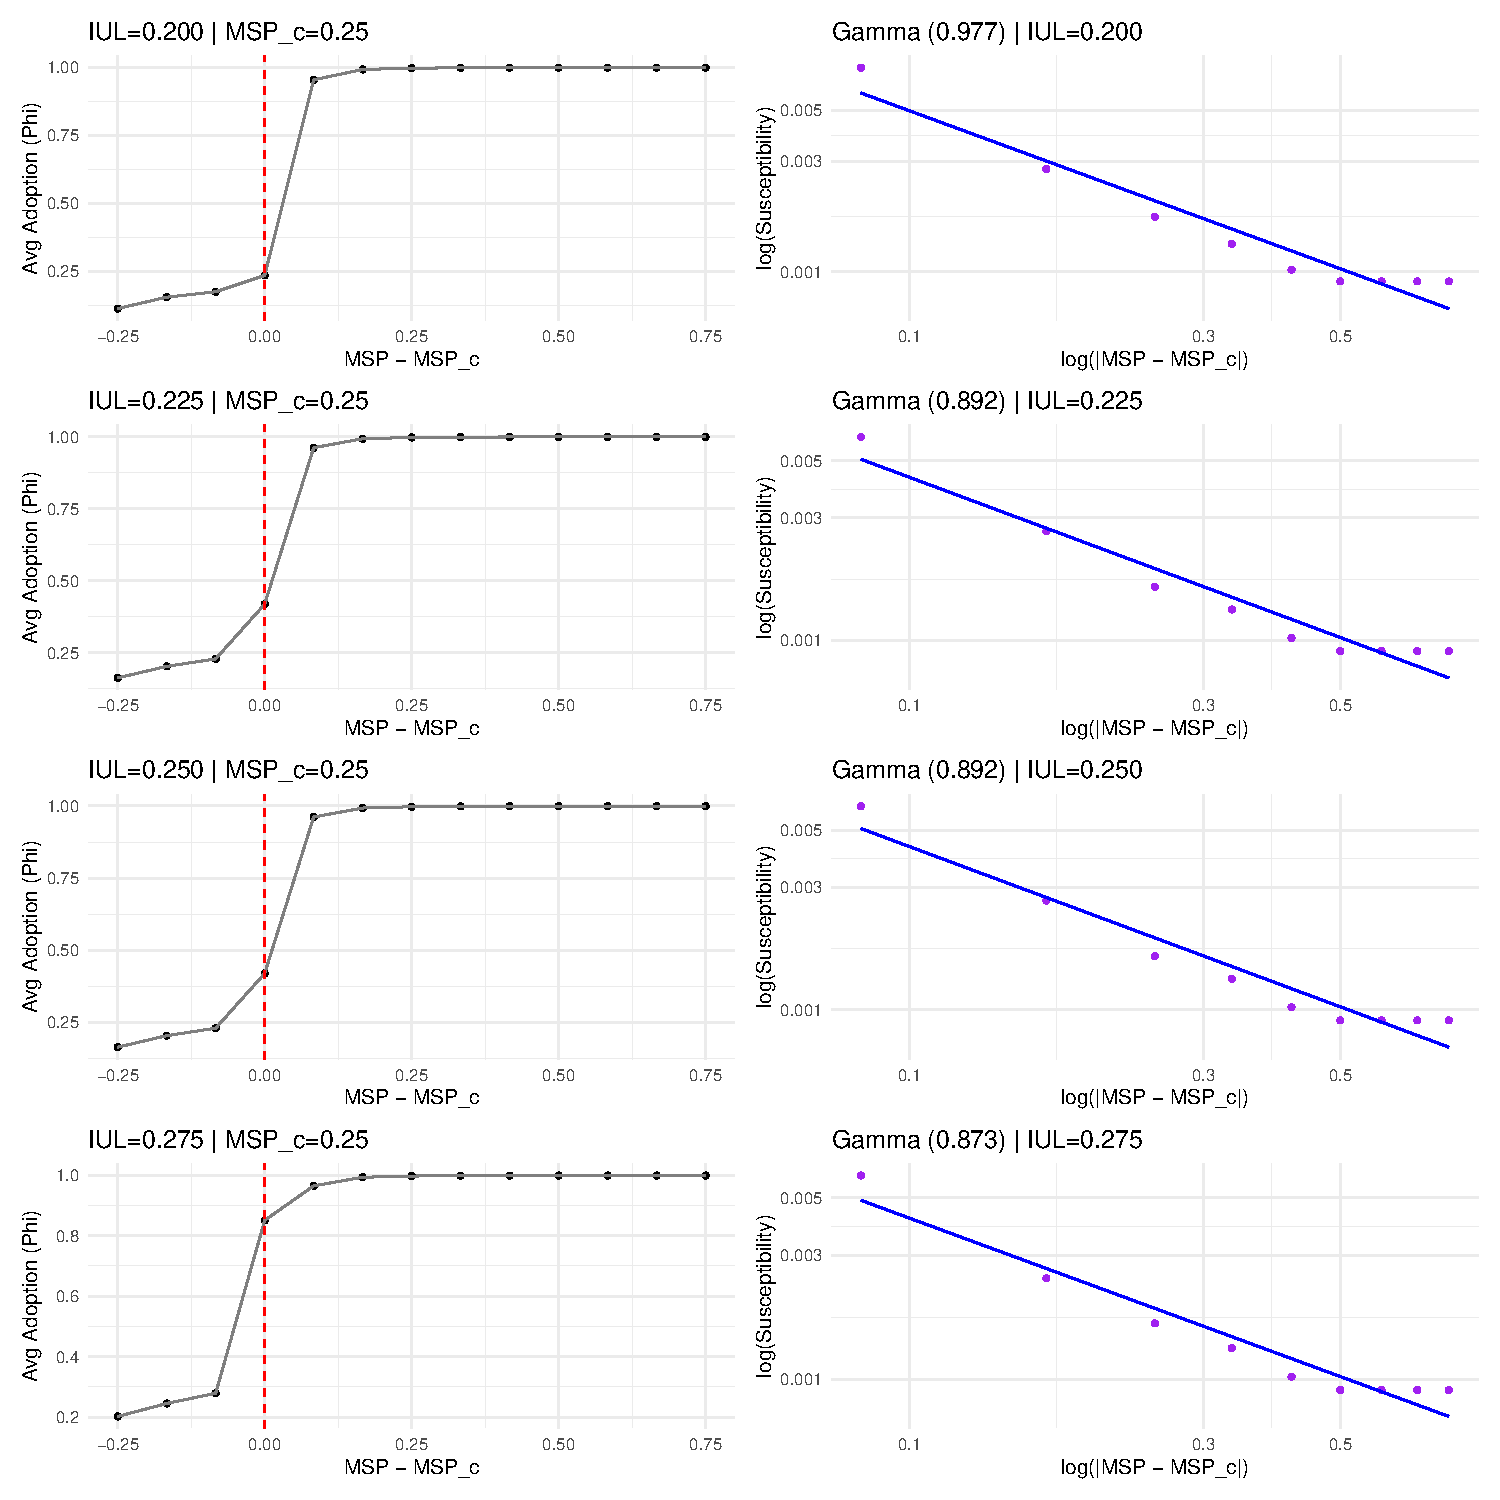
\includegraphics[width=1\textwidth]{../../plots/07_phase_transition/GSS/method4_exponents.pdf}
    \caption{\textbf{Critical Exponents (Method 4).} Log-log plots of the order parameter $\Phi$ (left panels) and susceptibility $\chi$ (right panels) against $|MSP - MSP_c|$ for four IUL values along the Widom Line. Linear fits in log-log space confirm power-law scaling with exponent $\gamma \approx 0.977$, consistent with Mean-Field universality.}
\end{figure}

\begin{table}[H]
\centering
\caption{\textbf{BAM Regression Results: Effect of Network Structure and Seeding.}}
\begin{tabular}{lccc}
\toprule
 & \textbf{Rational Adoption} & \textbf{Social Adoption} & \textbf{Total Adoption} \\
\midrule
(Intercept) & $0.428^{***}$ & $-0.300^{***}$ & $6.534^{***}$ \\
$\tau_{mean}$ & $-0.185^{***}$ & $-5.130^{***}$ & $-6.944^{***}$ \\
$\tau_{sd}$ & $0.032$ & $4.210^{***}$ & $5.942^{***}$ \\
\midrule
\textit{Seeding (Ref: Random)} & & & \\
Central & $-0.054^{***}$ & $0.032^{***}$ & $0.120^{***}$ \\
Closeness & $-0.052^{***}$ & $0.033^{***}$ & $0.119^{***}$ \\
Marginal & $0.027^{***}$ & $-0.020^{***}$ & $-0.067^{***}$ \\
\midrule
\textit{Structure (Ref: Plausible)} & & & \\
\textbf{Network: Random (ER)} & $\mathbf{-0.114^{***}}$ & $\mathbf{-0.426^{***}}$ & $\mathbf{-0.850^{***}}$ \\
\midrule
Deviance Explained & 96.9\% & 71.1\% & 82.2\% \\
\bottomrule
\multicolumn{4}{p{0.9\textwidth}}{\footnotesize $^{*}p<0.05, ^{**}p<0.01, ^{***}p<0.001$. Table includes all fixed effects from the reference model. Non-linear smooth terms $s(IUL, MSP)$ are highly significant ($p<0.001$).}
\end{tabular}
\end{table}

\begin{table}[H]
\centering
\caption{\textbf{Empirical Critical Exponents along the Widom Line.}}
\begin{tabular}{cc}
\toprule
\textbf{Intrinsic Utility (IUL)} & \textbf{Susceptibility Exponent ($\gamma$)} \\
\midrule
0.200 & 0.977 \\
0.225 & 0.892 \\
0.250 & 0.892 \\
0.275 & 0.873 \\
\bottomrule
\multicolumn{2}{p{0.55\textwidth}}{\footnotesize Mean-Field Ising prediction: $\gamma = 1.0$. Exponents estimated via OLS in log-log space along the super-critical arm of each Widom Line cross-section.}
\end{tabular}
\end{table}

\section*{Key References}
{\small
\noindent[1] Granovetter, M. (1978). Threshold models of collective behavior. \textit{American Journal of Sociology}, 83(6), 1420--1443.\\
\noindent[2] McPherson, M., \& Smith, J. A. (2019). Network effects in Blau space: Imputing social context from survey data. \textit{Socius}, 5, 2378023119865457.\\
\noindent[5] Sethna, J. P. (2021). \textit{Statistical Mechanics: Entropy, Order Parameters, and Complexity} (2nd ed.). Oxford University Press.\\
\noindent[6] Snijders, T. A., van de Bunt, G. G., \& Steglich, C. E. (2010). Introduction to stochastic actor-based models for network dynamics. \textit{Social Networks}, 32(1), 44--60.\\
\noindent[7] Tur, E. M., Zeppini, P., \& Frenken, K. (2024). Diffusion in small worlds with homophily and social reinforcement. \textit{Social Networks}, 76, 12--21.\\
\noindent[8] Valente, T. W. (1996). Social network thresholds in the diffusion of innovations. \textit{Social Networks}, 18(1), 69--89.\\
\noindent[9] Vega Yon, G., Olivera Morales, A., \& Valente, T. (2025). netdiffuseR: Analysis of Diffusion and Contagion Processes on Networks. \textit{zenodo}, doi:10.5281/zenodo.1039317.
}

\end{document}
